%!TEX TS-program = xelatex
%!TEX encoding = UTF-8 Unicode
\documentclass[11pt, letterpaper, oneside, extrafontsizes]{memoir}

\pagestyle{empty}


\usepackage{todonotes}
\usepackage{graphicx}

\usepackage[top=1in,bottom=1in,left=1.5in,right=1.5in]{geometry}

\begin{document}

\begin{center}
    \hspace*{\fill}
    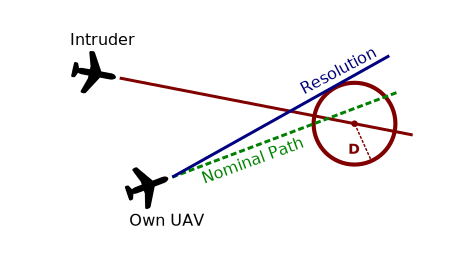
\includegraphics[height=3cm]{../media/simple_trl.pdf}
    \hfill{}
    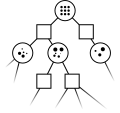
\includegraphics[height=3.5cm]{../media/pomcpow_tree.pdf}
    \hspace*{\fill}
    \\

    \vspace{0.5cm}
    \includegraphics[height=3cm]{../media/states.pdf}\\

    \vspace{0.5cm}
    \includegraphics[width=0.8\linewidth]{../media/cropped_julia18MVWL.png}

    \vspace{1cm}

    Doctoral Thesis Defense:\\
    \vspace{10pt}
    \textbf{\LARGE Safety and Efficiency in Autonomous Vehicles through Planning with Uncertainty}\\
    \vspace{10pt}
    Zachary Sunberg, Stanford Intelligent Systems Lab\\
    Department of Aeronautics and Astronautics\\
    May 25th, 2018, 9 AM, Room 200-205
\end{center}

Safety is the highest priority for autonomous vehicles, but if they are not also efficient in terms of time and other resources, they will have a significant competitive disadvantage and may not be adopted widely.
Though safety and efficiency are opposing goals, better models and planning algorithms can result in simultaneous improvements to both.
The partially observable Markov decision process (POMDP) provides a systematic framework for representing the chain of decisions that an autonomous vehicle makes when driving or flying.
However, it is challenging to find an optimal policy for POMDPs that represent continuous physical domains.

This dissertation analyzes and demonstrates improvements related to several aspects of making safe and efficient decisions.
First, it considers how pseudo-random approximate algorithms can be combined with trusted deterministic algorithms to make certification easier and increase reliability.
Second, simulation results demonstrate that modeling uncertainty in the internal states of other road users in highway lane-changing using POMDP planning can lead to significant improvement over a formulation that models only outcome uncertainty.
Finally, the research shows that current leading online POMDP algorithms are unable to solve some problems with continuous observation spaces, and overcomes this weakness using double progressive widening and weighted particle filtering.

% \includegraphics[width=10in]{some-fig.jpg}

\end{document}
